\documentclass{article}

% 导入宏包
\usepackage{fancyhdr}
\usepackage{ctex}
\usepackage{listings}
\usepackage{graphicx}
\usepackage[a4paper, body={18cm,22cm}]{geometry}
\usepackage{amsmath,amssymb,amstext,wasysym,enumerate,graphicx}
\usepackage{float,abstract,booktabs,indentfirst,amsmath}
\usepackage{array}
\usepackage{multirow}
\usepackage{url}
\usepackage{diagbox}
\usepackage{enumitem}
\usepackage{xcolor}
\usepackage{makecell}
\usepackage{tikz}
\usetikzlibrary{positioning, arrows.meta}

% 设置段落
\renewcommand\arraystretch{1.4}
\setlength{\parindent}{2em}
\setCJKmonofont{黑体}

% 配置代码显示
\lstset{
	xleftmargin = 3em,
	xrightmargin = 3em,
	aboveskip = 1em,
	backgroundcolor = \color{white},
	basicstyle = \small\ttfamily,
	rulesepcolor = \color{gray},
	breaklines = true,
	numbers = left,
	numberstyle = \small,
	numbersep = -14pt,
	keywordstyle = \color{purple}\bfseries,
	commentstyle = \color{green!60!black}, % 修改注释颜色
	stringstyle = \color{red!60!green!90!blue!90},
	morekeywords = {ASSERT, int64_t, uint32_t},
	moreemph = {ASSERT, NULL},
	emphstyle = \color{red}\bfseries,
	moreemph = [2]{int64\_t, uint32\_t, tid\_t, uint8\_t, int16\_t, uint16\_t, int32\_t, size\_t, bool},
	emphstyle = [2]\color{purple}\bfseries,
	frame = shadowbox,
	showspaces = false,
	columns = fixed
	morecomment = [l][\color{green!60!black}]{+}, % 设置以+开头的代码行为绿色
}

%--------------------页眉--------------------%

\pagestyle{fancy}
\fancyhead[L]{}
\fancyhead[R]{}
\fancyhead[C]{华东师范大学软件工程学院实验报告}
\fancyfoot[C]{-\thepage-}
\renewcommand{\headrulewidth}{1.5pt}

%--------------------标题--------------------%

\begin{document}
	\begin{center}
		{\Large{\textbf{\heiti 华东师范大学软件工程学院实验报告}}}
		\begin{table}[htb]
			\flushleft
			\begin{tabular}{p{0.4\linewidth}p{0.27\linewidth}p{0.28\linewidth}}\\
				\textbf{实验课程}:计算机网络实践  & \textbf{年级}:2023级       & \textbf{实验成绩}:  \\
				\textbf{实验名称}:UDP & \textbf{姓名}:顾翌炜         &                 \\
				\textbf{实验编号}:Lab-5     & \textbf{学号}:10235101527 & \textbf{实验日期}:2024/12/20  \\
				\textbf{指导教师}:王廷     & \textbf{组号}:01            & \textbf{实验时间}:2024/12/20  \\ 
			\end{tabular}
		\end{table}
	\end{center}
	\rule{\textwidth}{2pt}
	
	%--------------------正文--------------------%
	\section{实验目的}
	
	\begin{enumerate}[noitemsep, label={{\arabic*})}]
		\item 学习使用Wireshark抓取UDP数据包
		\item 理解UDP数据包的结构
		\item 熟悉UDP数据包中各个字段的含义
		\item 掌握UDP协议的应用场景
	\end{enumerate}
	
	\section{实验内容与实验步骤}
	
	\subsection{实验内容}
	
	\begin{enumerate}[noitemsep, label={{\arabic*})}]
		\item 学会通过Wireshark获取UDP消息
		\item 掌握UDP数据包结构
		\item 掌握UDP数据包各字段的含义
		\item 了解UDP协议适用领域
	\end{enumerate}\textbf{}
	
	\subsubsection{获取 \texttt{UDP} 消息}
	
	打开 \texttt{Wireshark},在“捕获”菜单中选择“选项”,配置以太网接口,设置捕获过滤器为 \texttt{udp},并关闭混杂模式。
	
	点击“开始”按钮,使用浏览器访问一个网站,如 \texttt{www.baidu.com},
	或在命令行中输入 \texttt{nslookup www.baidu.com} 查询DNS服务器。
	如果DNS解析失败,可以在命令行中输入 \texttt{ipconfig /flushdns} 清除 \texttt{DNS} 缓存。
	( 使用 \texttt{ipconfig /displaydns} 可以在 \texttt{Windows} 系统中查看当前的 \texttt{DNS} 缓存)
	
	完成捕获后,点击“停止”按钮。
	
	\subsubsection{分析 \texttt{UDP} 包}
	选择一个数据帧,分析其\texttt{UDP}包头字段。
	
	回答以下问题:
	
	\begin{enumerate}[label={\arabic*})]
		\item What does the Length field include? The UDP payload, UDP payload and UDP header, or UDP payload, UDP header, and lower layer headers?
		\item How long in bits is the UDP checksum?
		\item How long in bytes is the entire UDP header? 
	\end{enumerate}
	
	打开命令行界面,输入 \texttt{ipconfig} 以获取计算机的 \texttt{IP} 地址,并将其与数据包中的 \texttt{Source Port} 进行比较。
	
	回答以下问题:
	
	\begin{enumerate}[label={\arabic*})]
		\item Give the value of the IP Protocol field that identifies the upper layer protocol as UDP.
		
		\item Examine the UDP messages and give the destination IP addresses that are used when your computer is neither the source IP address nor the destination IP address. (If you have only your computer as the source or destination IP address then you may use the supplied trace.)
		
		\item What is the typical size of UDP messages in your trace?
	\end{enumerate}
	
	\subsubsection{问题讨论}
	
	We encourage you to keep exploring on your own, but there is not much more to UDP. 
	
	Instead, you might examine the traffic of UDP-based applications to look at packet sizes and loss rates. Voice-over-IP and its companion protocols like RTP (Real-Time Protocol) are good candidates. 
	
	Similarly, you might explore streaming and real-time applications to see which use UDP and which use TCP as a transport.
	
	\subsection{实验步骤}
	
	\begin{enumerate}[noitemsep, label={{\arabic*})}]
		\item 启动 \texttt{Wireshark},在“捕获” $\to$ “选项”中进行设置,选择已连接的以太网接口,将捕获过滤器设置为 \texttt{udp},并关闭混杂模式,然后开始捕获。
		\item 在命令行中输入 \texttt{nslookup www.baidu.com} 查询 \texttt{DNS} 服务器
		
		\begin{lstlisting}
			PS> nslookup www.baidu.com
		\end{lstlisting}
		\item 在 \texttt{Wireshark} 中停止捕获。
		\item 对捕获到的 \texttt{UDP} 数据包进行分析,并回答相关问题。
		\item 讨论问题
	\end{enumerate}
	
	\section{实验环境}
	
	\begin{itemize}[noitemsep]
		\item 操作系统:\texttt{Windows 11 家庭中文版 23H2 22631.4460}
		\item 网络适配器:\texttt{Killer(R)Wi-Fi 6E AX1675i 160MHz Wireless Network Adapter(211NGW)}
		\item \texttt{Wireshark}:\texttt{Version 4.4.1}
		\item \texttt{wget}:\texttt{GNU Wget 1.21.4 built on mingw32}
	\end{itemize}
	
	\section{实验结果与分析}
	
	\subsection{获取UDP消息}
	
	打开Wireshark,在菜单栏的捕获的选项中进行设置,选择已连接的以太网,设置捕获过滤器为udp,关闭混杂模式。
	
	\begin{figure}[H]
		\centering
		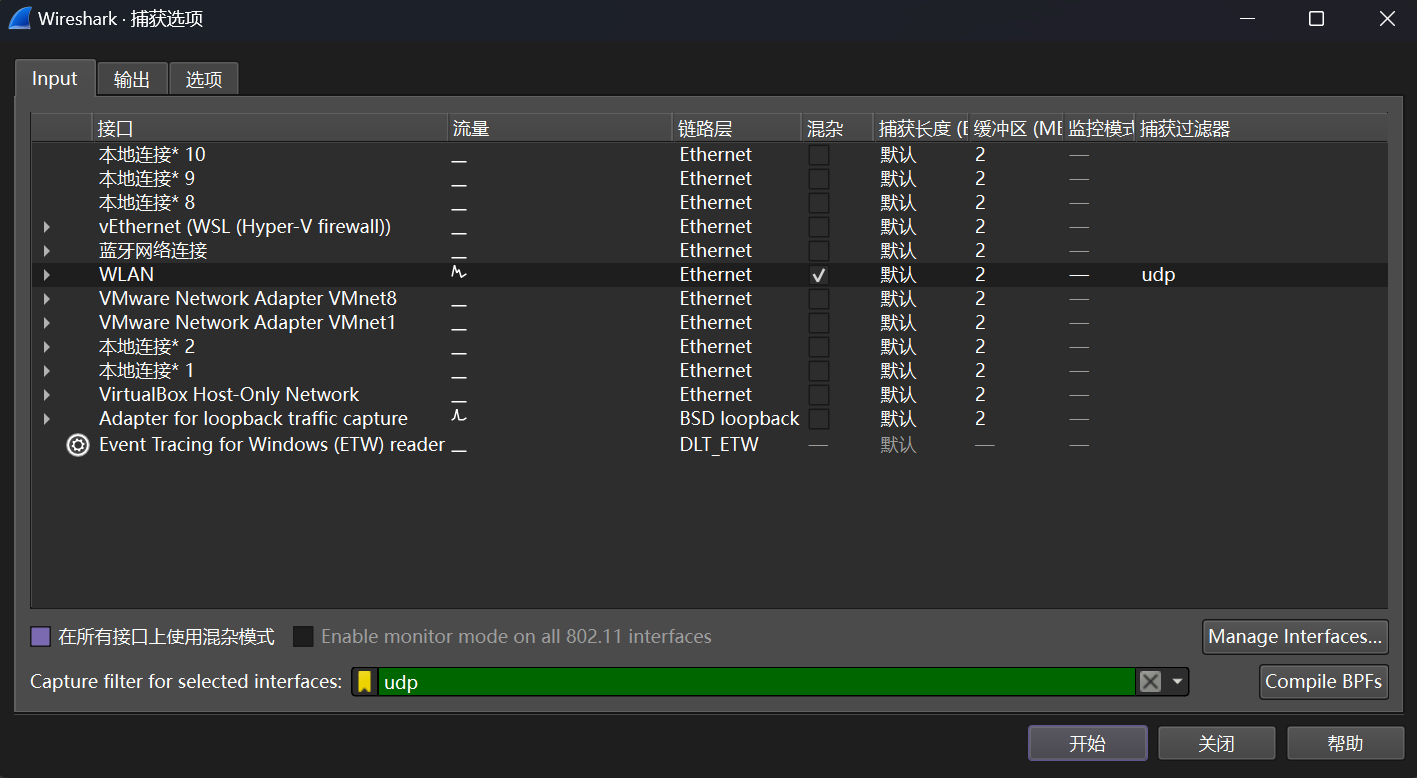
\includegraphics[width=11cm]{images/1.设置捕获.png}
		\caption{设置捕获}
	\end{figure}
	
	开始捕获,在cmd中输入 \texttt{nslookup www.baidu.com} 查询DNS服务器
	
	\begin{figure}[H]
		\centering
		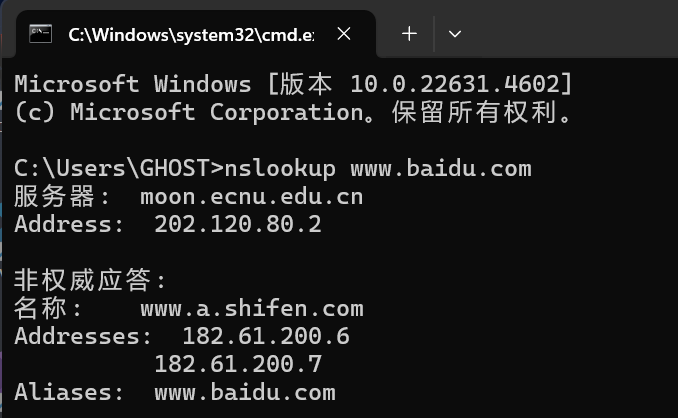
\includegraphics[width=11cm]{images/2.查询DNS服务器.png}
		\caption{查询DNS服务器}
	\end{figure}
	
	得到的捕获结果如下所示:
	
	\begin{figure}[H]
		\centering
		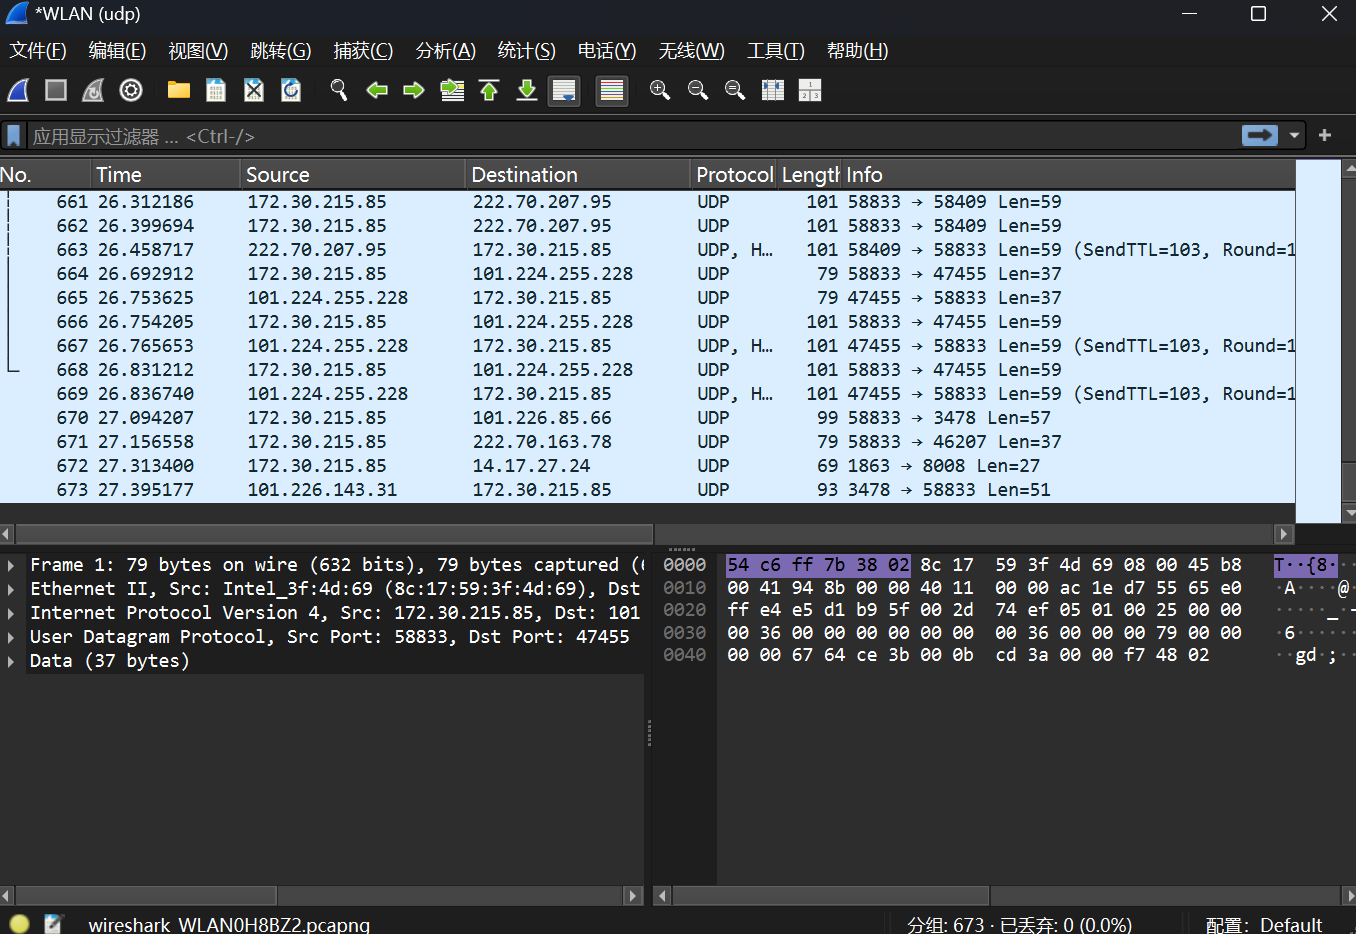
\includegraphics[width=11cm]{images/3.捕获结果.png}
		\caption{捕获结果}
	\end{figure}
	
	由此,捕获UDP的部分就结束了。
	
	\subsection{分析UDP包}
	
	从捕获结果中选择一个数据帧,分析其UDP包头字段。
	
	\begin{figure}[H]
		\centering
		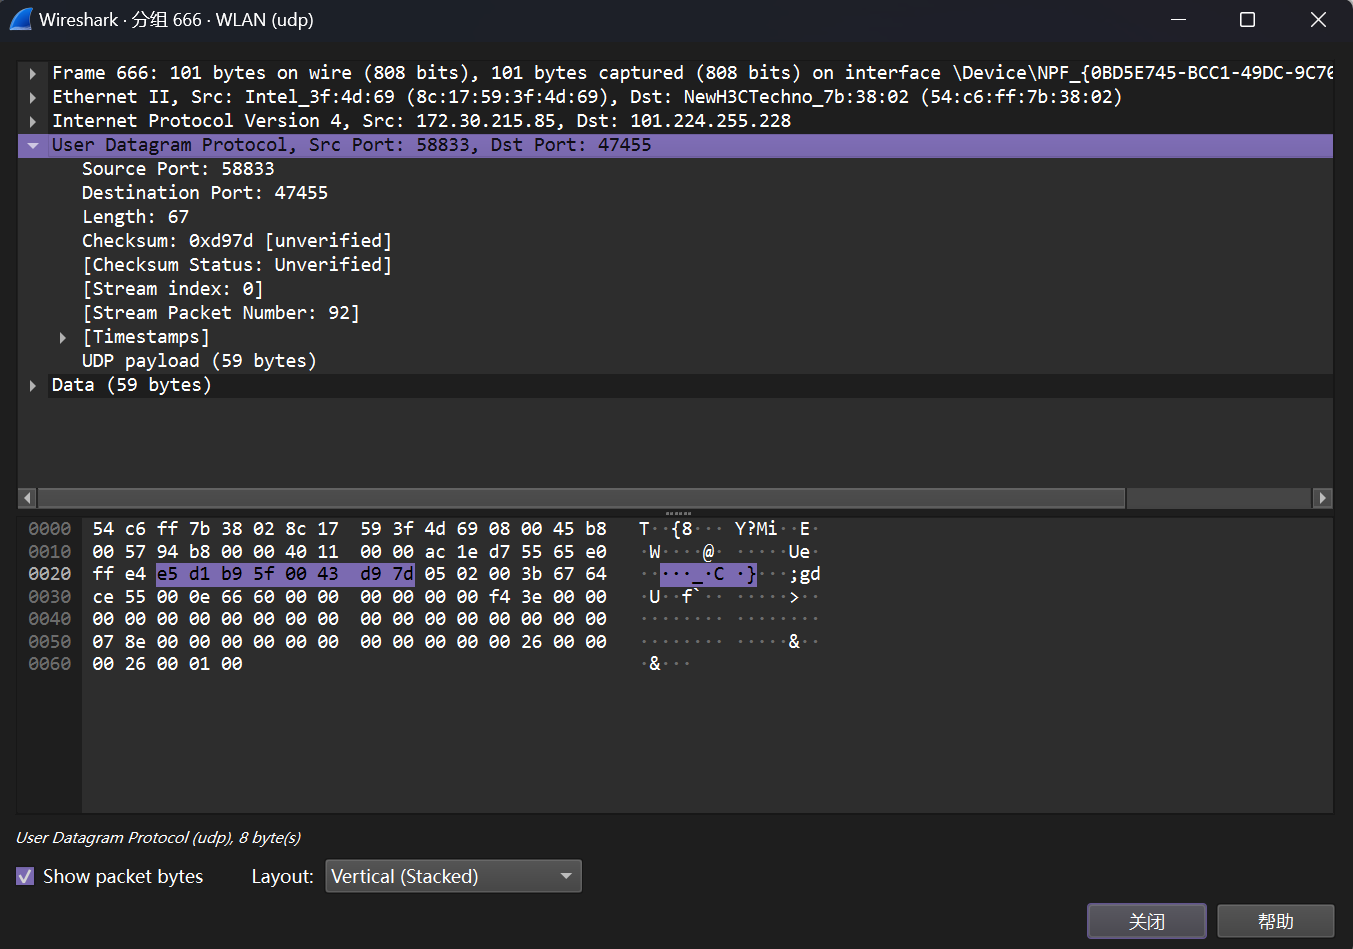
\includegraphics[width=11cm]{images/4.UDP包.png}
		\caption{UDP包}
	\end{figure}
	
	来看UDP包的每一个部分:
	
	\begin{figure}[H]
		\centering
		\begin{minipage}[b]{0.45\textwidth}
			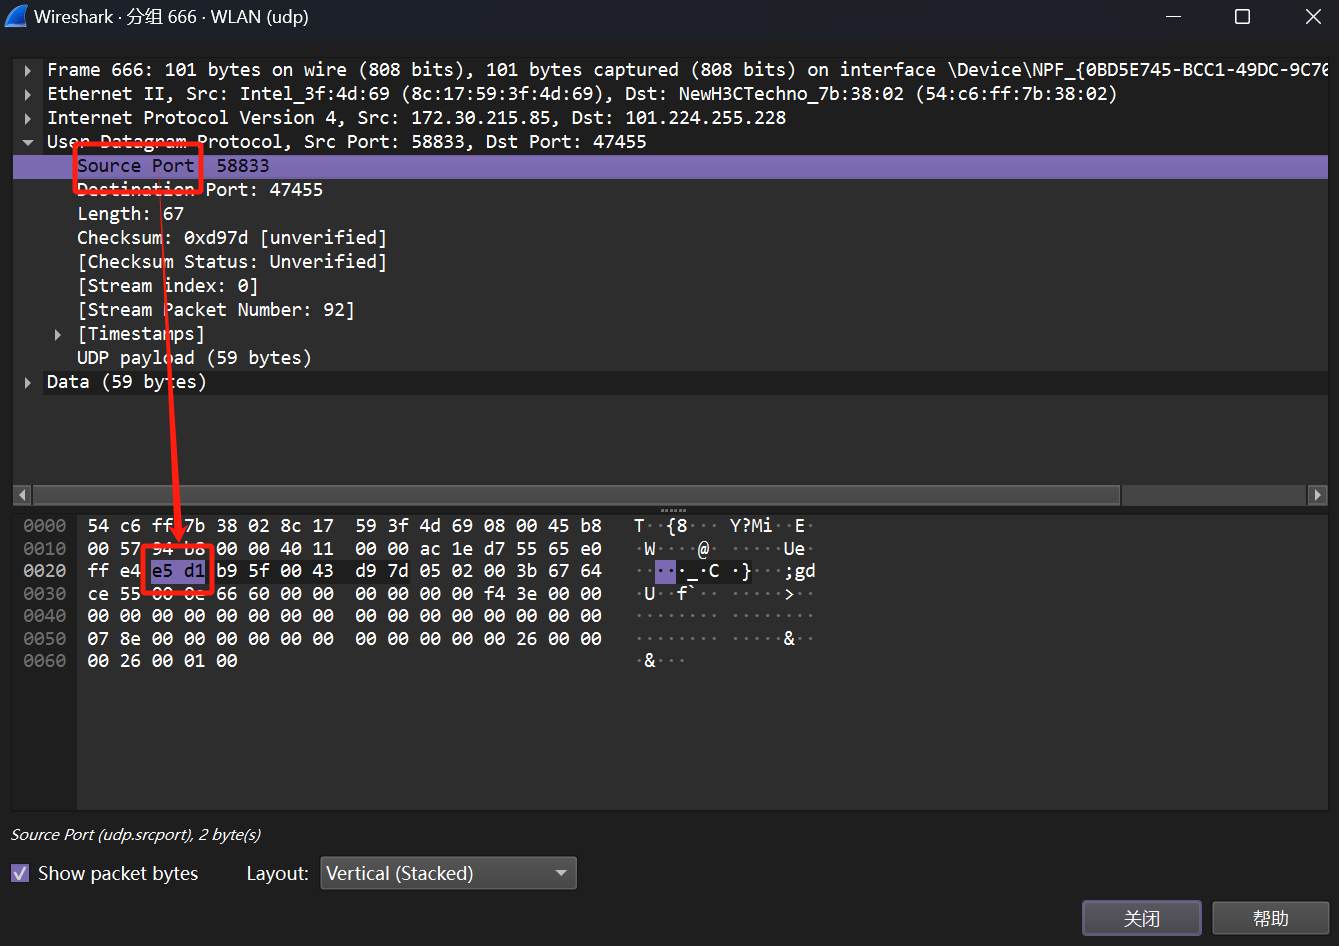
\includegraphics[width=\textwidth]{images/5.Source Port.png}
			\caption{Source Port}
		\end{minipage}
		\hfill
		\begin{minipage}[b]{0.45\textwidth}
			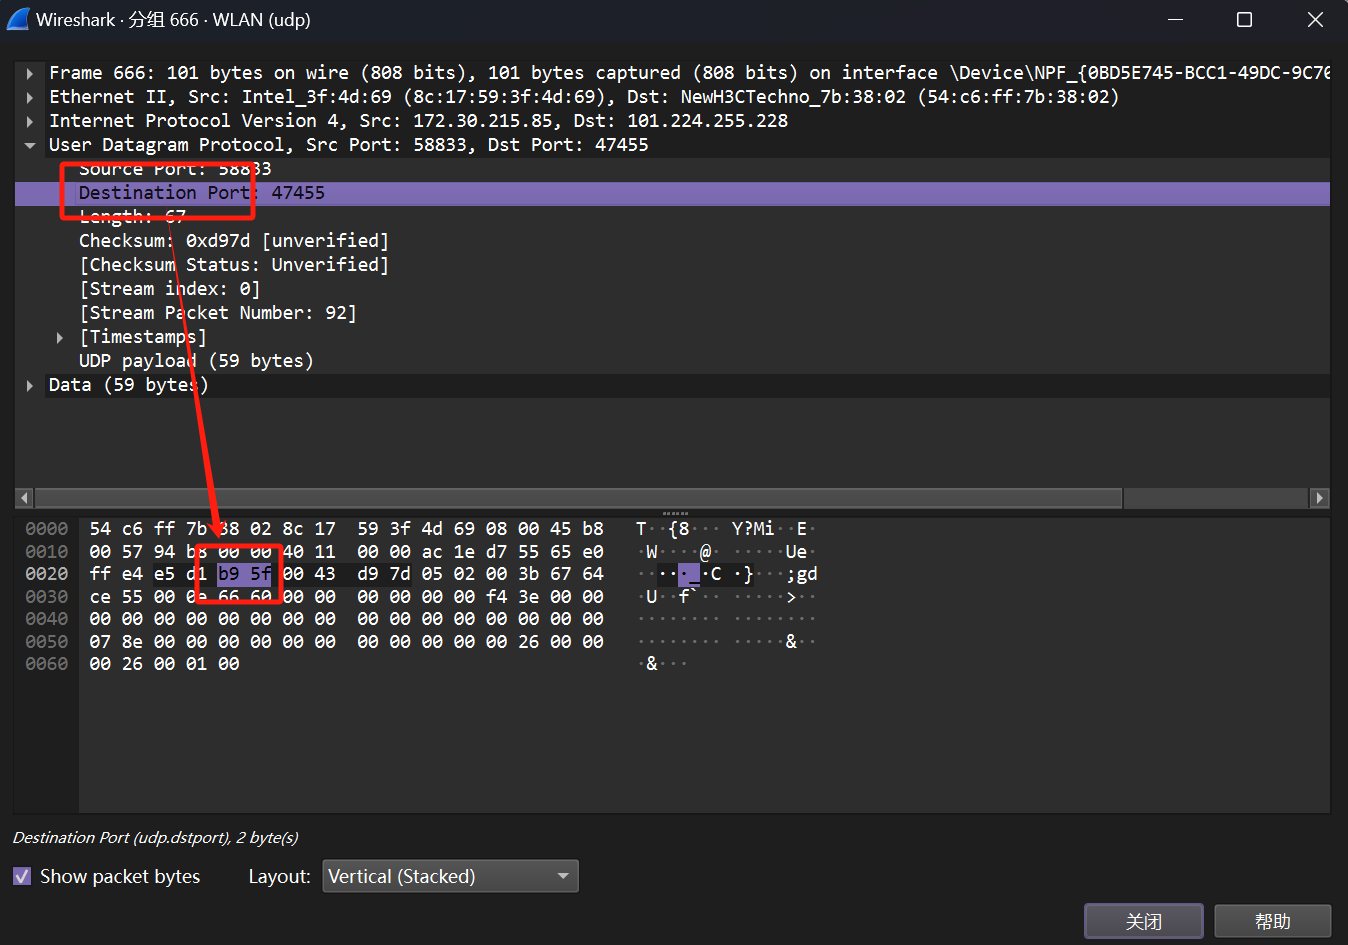
\includegraphics[width=\textwidth]{images/6.Destination Port.png}
			\caption{\texttt{Destination Port}}
		\end{minipage}
	\end{figure}
	
	\begin{figure}[H]
		\centering
		\begin{minipage}[b]{0.45\textwidth}
			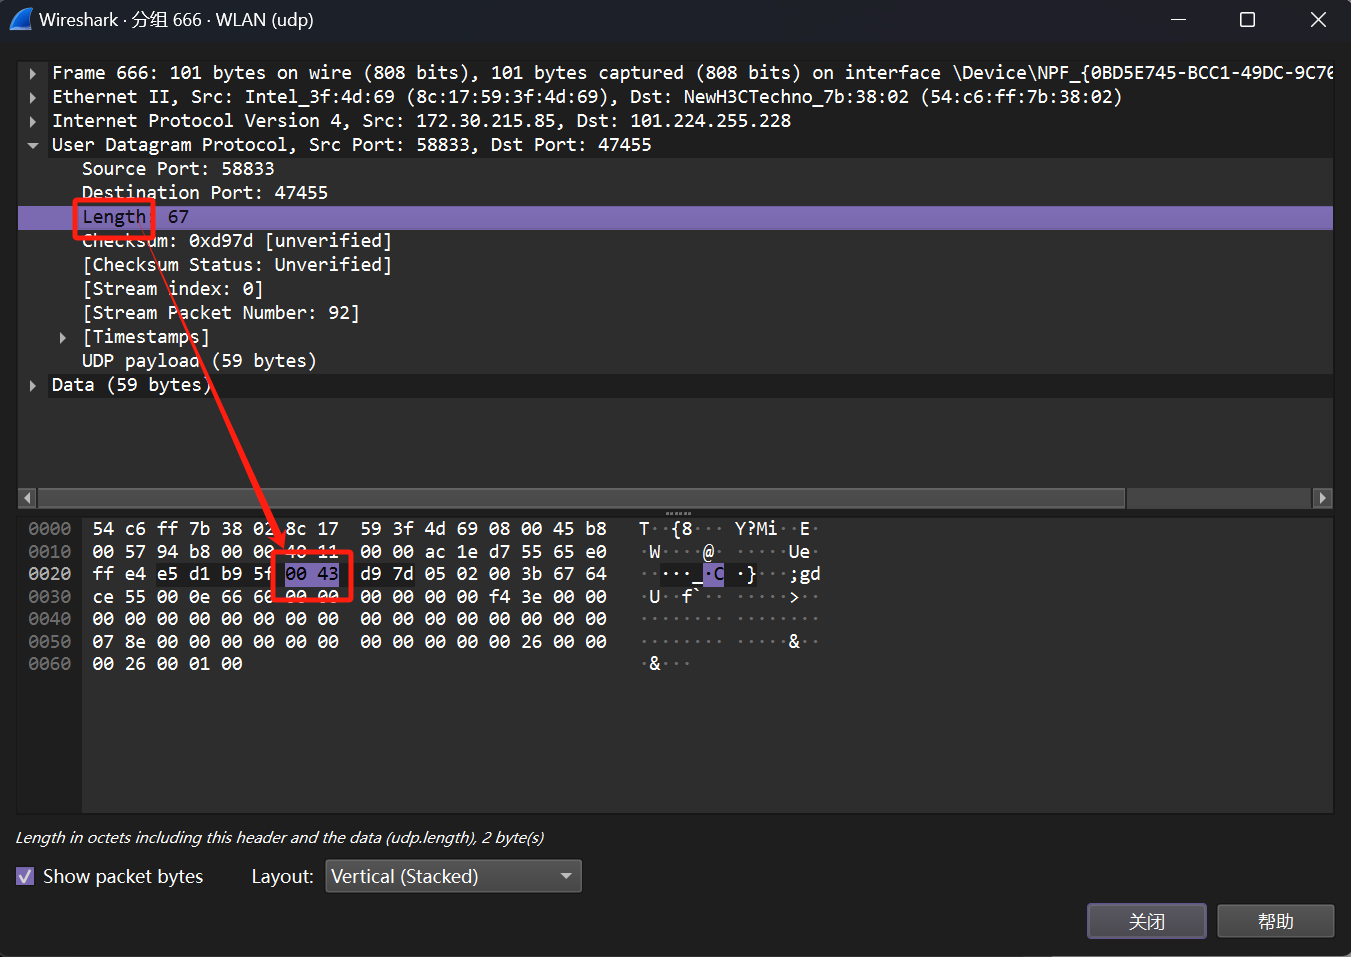
\includegraphics[width=\textwidth]{images/7.Length.png}
			\caption{Length}
		\end{minipage}
		\hfill
		\begin{minipage}[b]{0.45\textwidth}
			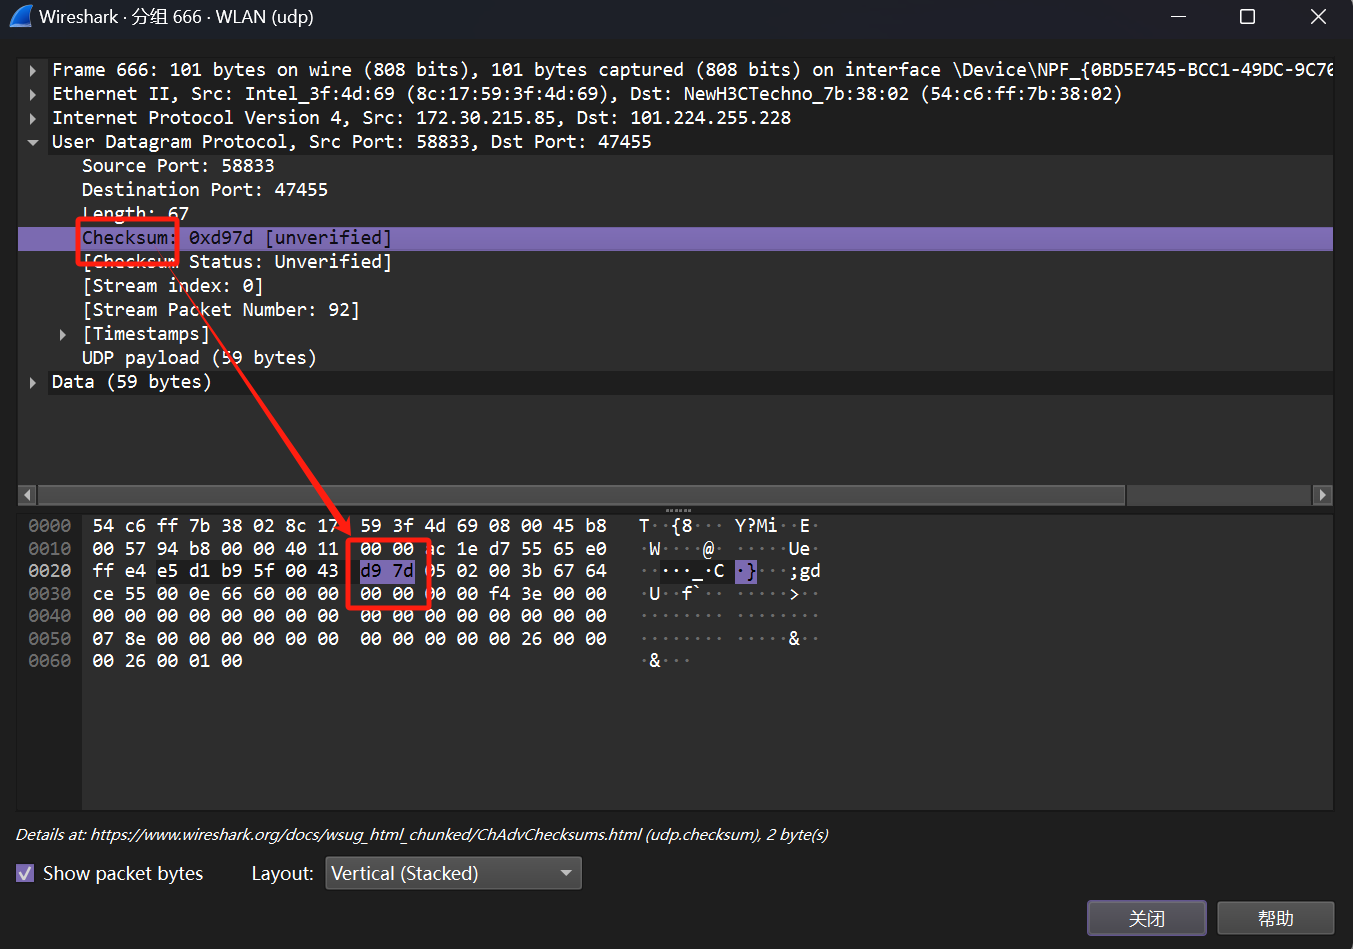
\includegraphics[width=\textwidth]{images/8.Checksum.png}
			\caption{\texttt{Checksum}}
		\end{minipage}
	\end{figure}
	
	由此可以画出UDP包的结构如下:
	
	\begin{figure}[H]
		\centering
		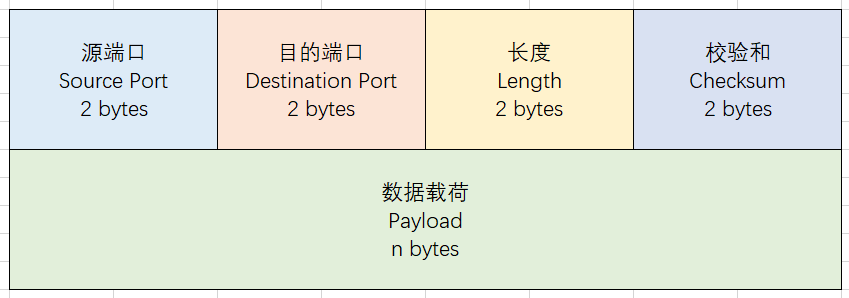
\includegraphics[width=11cm]{images/9.UDP包的结构.png}
		\caption{UDP包的结构}
	\end{figure}
	
	\subsection{回答问题}
	
	\begin{enumerate}[label={\arabic*})]
		\item What does the Length field include? The UDP payload, UDP payload and UDP header, or UDP payload, UDP header, and lower layer headers?
		
		在上面分析的UDP包中,Payload长度为59字节,UDP 头长度为8字节,而Length字段的值为67。
		
		因此可以得出UDP 数据报头中的Length 字段指的是UDP的payload长度加上UDP头的总长度。
		
		\item How long in bits is the UDP checksum?
		
		UDP头中的checksum的长度是16 位。
		
		\item How long in bytes is the entire UDP header? 
		
		整个UDP头的长度是8字节。
	\end{enumerate}
	
	打开命令行界面,输入 \texttt{ipconfig} 以获取计算机的 \texttt{IP} 地址,并将其与数据包中的 \texttt{Source Port} 进行比较。
	
	可以看到我的ip地址是:
	
	\begin{figure}[H]
		\centering
		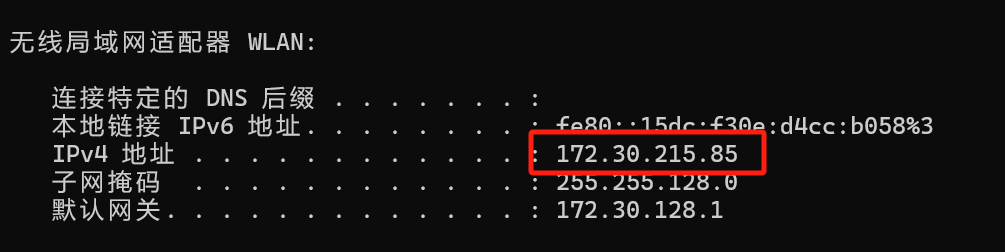
\includegraphics[width=11cm]{images/10.IP地址.png}
		\caption{IP地址}
	\end{figure}
	
	可以看到我的ip地址是 \texttt{172.30.215.85} ,与数据报中的Source Port = 58833相同,与数据报中的Destination Port = 47455不同
	
	回答以下问题:
	
	\begin{enumerate}[label={\arabic*})]
		\item Give the value of the IP Protocol field that identifies the upper layer protocol as UDP.
		
		在IP协议中,Protocol字段指出需要交给上一层的UDP传输进程,该字段值为17。
		
		\begin{figure}[H]
			\centering
			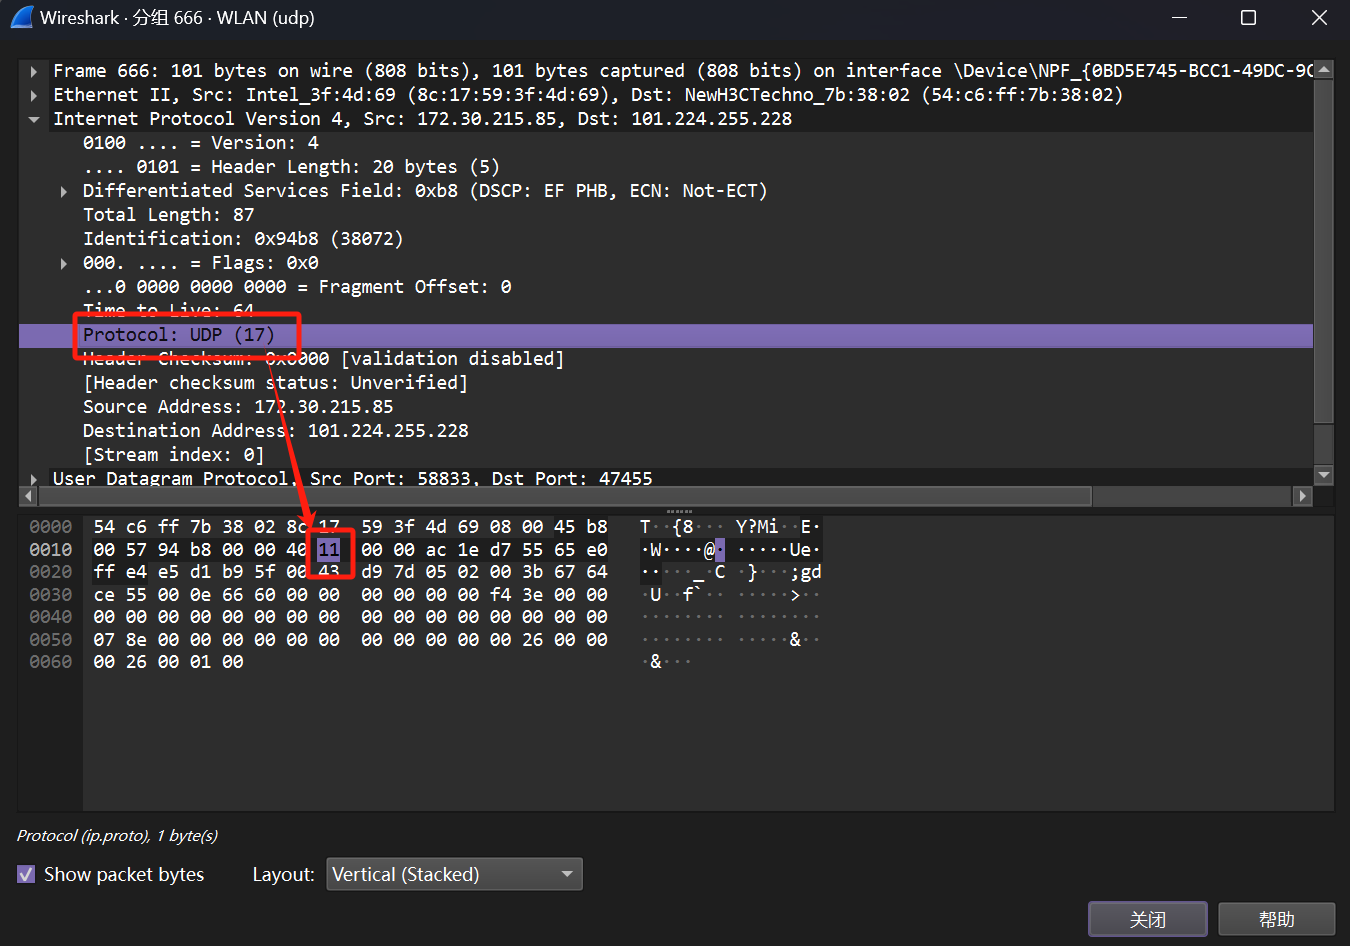
\includegraphics[width=11cm]{images/11.Protocol.png}
			\caption{Protocol}
		\end{figure}
		
		\item Examine the UDP messages and give the destination IP addresses that are used when your computer is neither the source IP address nor the destination IP address. (If you have only your computer as the source or destination IP address then you may use the supplied trace.)
		
		\begin{figure}[H]
			\centering
			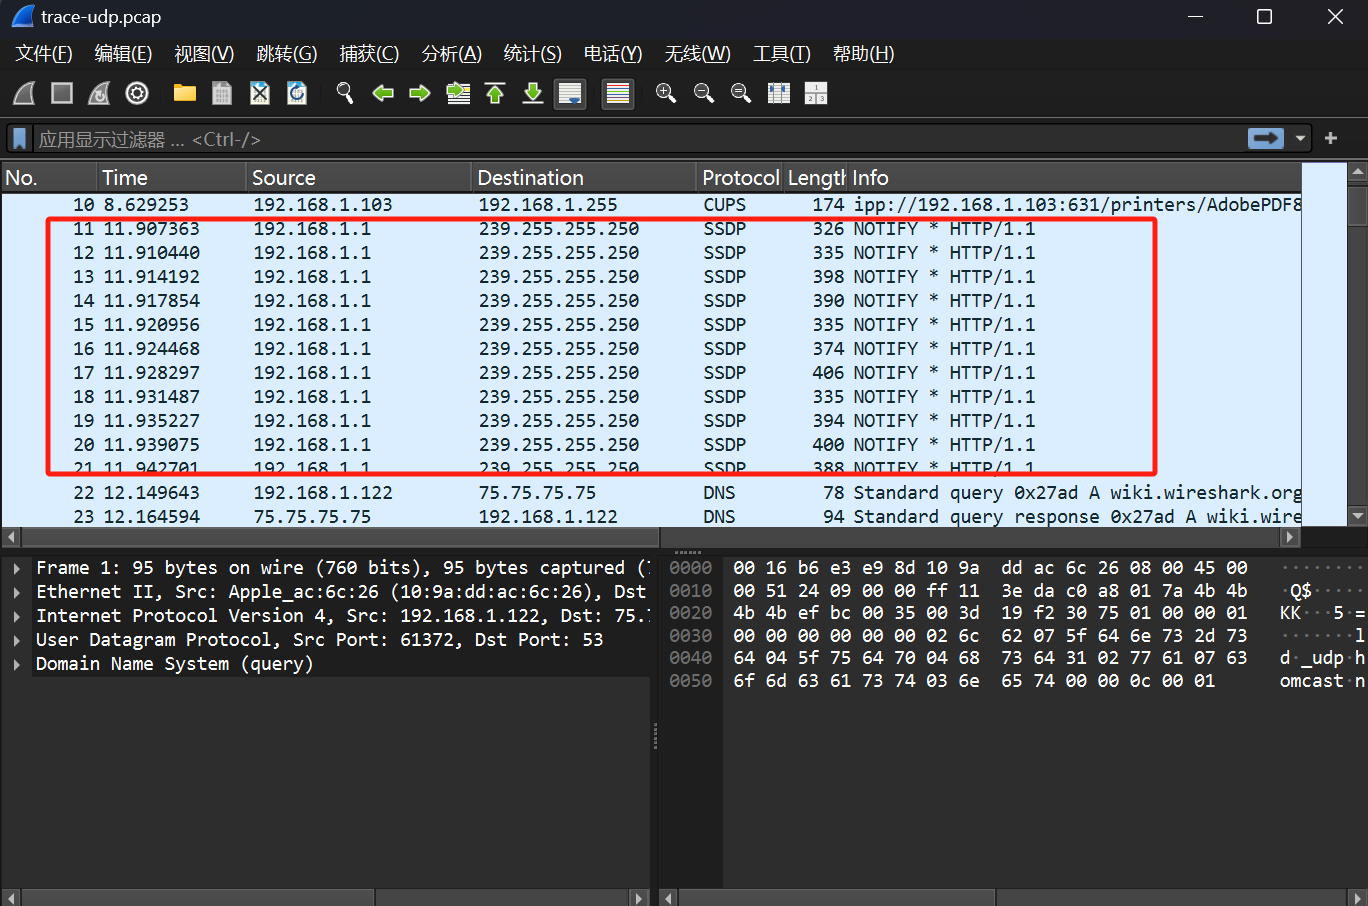
\includegraphics[width=11cm]{images/12.数据包.png}
			\caption{数据包}
		\end{figure}
		
		可以看到,这些数据包的 destination IP 地址为239.255.255.250
		
		\item What is the typical size of UDP messages in your trace?
		
		由于UDP报头中的Length字段为2字节,因此最大长度可达到$2^{16} - 1$字节,即65535字节。然而,考虑到以太网帧的最大载荷为1500字节,而IP报头为20字节,这意味着UDP消息的总长度不应超过1480字节。
		
	\end{enumerate}
	
	\subsection{问题讨论}
	
	We encourage you to keep exploring on your own, but there is not much more to UDP. Instead, you might examine the traffic of UDP-based applications to look at packet sizes and loss rates. Voice-over-IP and its companion protocols like RTP (Real-Time Protocol) are good candidates. 
	
	此处以QQ为例,QQ采用的是OICQ协议,这是基于UDP的,因此可以捕获QQ的数据包来分析

	\begin{figure}[H]
		\centering
		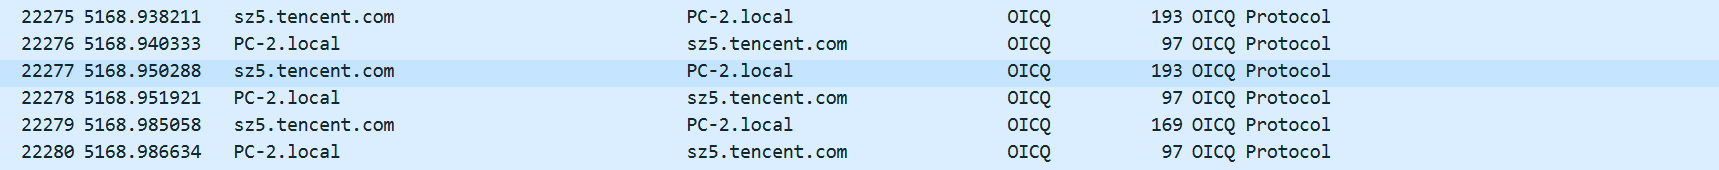
\includegraphics[width=11cm]{images/13.OICQ数据包.png}
		\caption{OICQ数据包}
	\end{figure}
	
	选择一个OICQ 数据包。
	
	\begin{figure}[H]
		\centering
		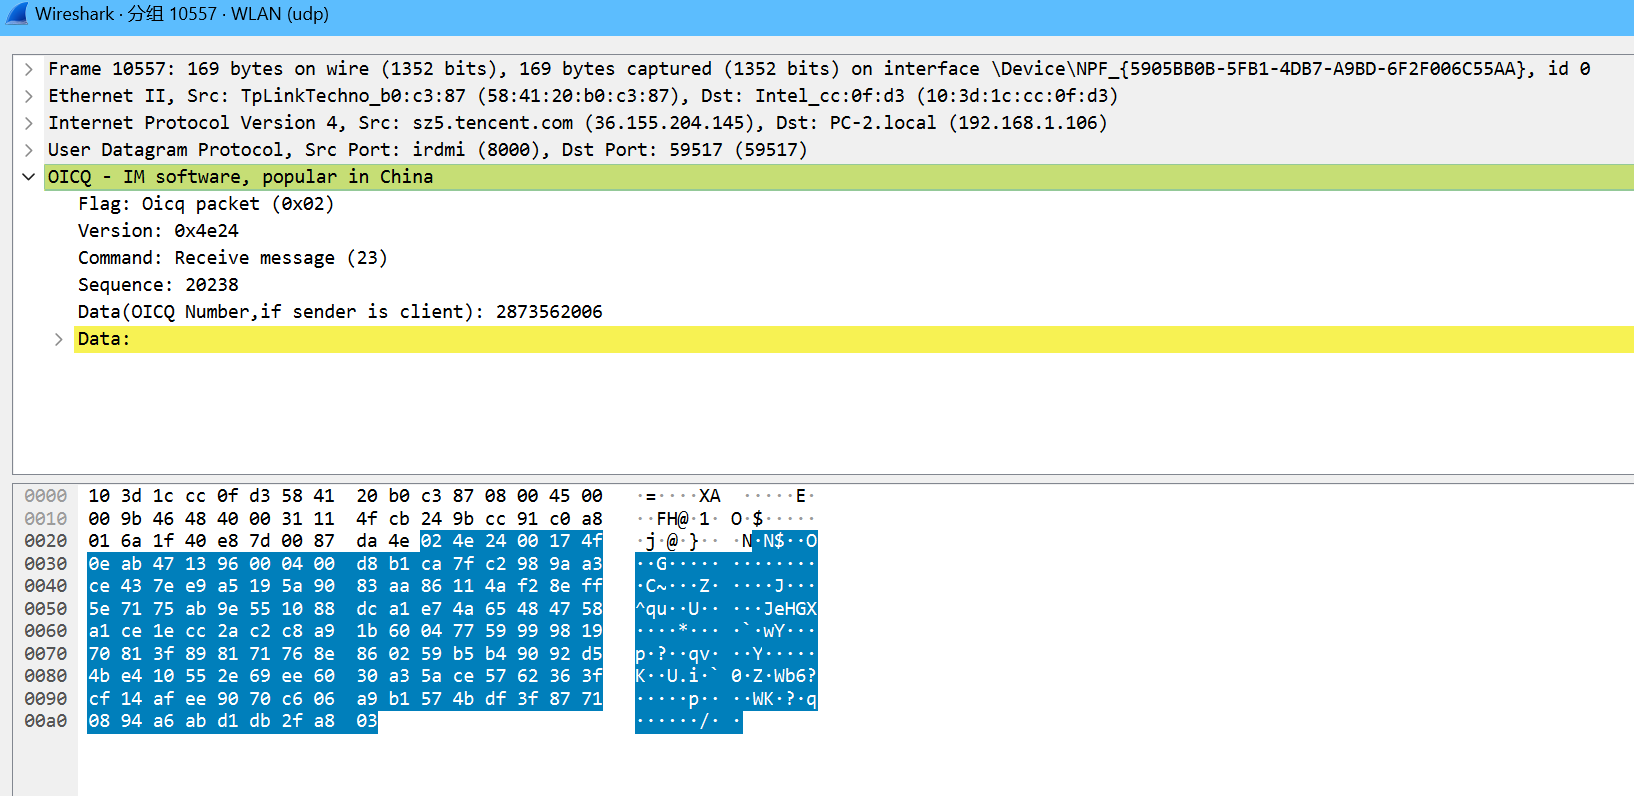
\includegraphics[width=11cm]{images/14.打开OICQ.png}
		\caption{打开OICQ}
	\end{figure}
	
	可以看到,OICQ 数据包的长度为647 字节。
	
	Similarly, you might explore streaming and real-time applications to see which use UDP and which use TCP as a transport.
	
	由于文件传输需要确保数据的完整性,因此通常采用TCP协议。相比之下,流媒体传输和实时通信可以使用UDP协议,因为这些应用对数据的实时性要求更高,偶尔的数据包丢失不会对其产生显著影响。
	
	\section{实验结果总结}
	
	通过本次实验,我学会了使用 \texttt{Wireshark} 捕获 \texttt{UDP} 消息,掌握了 \texttt{UDP} 数据包的结构,理解了各字段的含义,了解了 \texttt{UDP} 协议的应用场景。
	
	\section{附录}
	
	无
\end{document}